\chapter{基于信息熵的数据定价研究}

\section{研究动机}
近些年来,数据量的巨幅增长,尤其是从2005年到2010年,全球产生的数据量增长了10倍(从130艾字节增长到了1227艾字节),目前仍在继续增长\cite{gantz2012digital,villars2011big}。数据交易的市场也以惊人的速度发展着,预计从目前到2020年,大数据和其商业分析的市场规模会从1301亿美元增长到2030亿美元\cite{idc}。如今,高质量和可信赖的数据商品及其相关的分析业务有着巨量的市场需求\cite{gantz2012digital,maitland2002european,turner2014digital,villars2011big}。

现在,数据商品和相关分析业务主要是由在线数据市场提供的。这些市场从数据发布者和全球网络收集数据,并对其进行清洗、挖掘和整理,然后出售给不同的消费者。具体来说,数据消费者主要由开发者和中小企业主构成。这些数据消费者需要在线数据市场提供的数据和相关分析业务来帮助他们做商业决策。至于在线数据市场,他们在整理过的、有价值的数据的基础上,提供分析、商业应用和算法等服务给消费者。现在,国外主要有三家数据交易平台,分别是Microsoft Windows Azure Data Marketplace\cite{MicrosoftAzure}, Inforchimps\cite{infochimps}以及Factual\cite{factual}。而国内也主要有三家平台,分别是贵阳大数据交易所\cite{gbdex},武汉长江大数据交易中心和武汉东湖大数据交易中心\cite{chinadatatrading}。然而,在这些国内外数据交易平台,并没有一个统一的定价机制来指导整个市场。因此,当前数据产品的定价处于一个比较混乱的阶段。不同的数据交易平台采用的是不同的定价机制,而其中最普遍采用的有四种种机制:基于订阅的定价机制、基于查询的定价机制,捆绑销售定价机制以及私下协商定价机制。选择什么样的定价机制具体取决于消费者使用模式以及数据提供商之间的竞争差异。但是,需要指出的是,目前没有任何一种定价机制将数据本身所含有的信息量考虑为定价因素。从消费者角度考虑,目前很多数据消费者通常只对市场上数据集的某些子集感兴趣,他们并不需要购买完整的数据集,而交易平台往往给出的是完整数据集的价格。当消费者购买这些子集时,他们需要知道这些子集所含信息占完整数据集的比例从而评估交易平台给出的子集定价是否合理。从数据交易平台的角度看,如果他们能给出更多的子集数据价格以及它们之间的信息量关系的话,就能给消费者提供一个更加透明的定价关系,从而吸引更多的消费者进行消费。另一方面,目前已有的定价机制并不能产生最大交易剩余,这样会降低买卖双方的交易信心,从而使原本能发生的交易而没有发生,这将会对数据及其相关交易带来极大的经济损失。因此,我们进行了基于信息熵的数据交易的研究课题,期望以数据产品本身的信息量作为定价指标来更好地指导数据交易。

\section{定价策略与模型}

在本小节中,我们首先会给出基于信息熵数据定价的问题定义。然后针对这一问题,提出了基于信息熵数据定价的通用模型,并讨论了相关的性质和应用范围。

\subsection{问题定义}

如今,大部分工业界收集到的数据都是非结构化的。即使这些非结构化的数据能用矩阵形式表示,但是人们还是很难从这些数据结构中认识到结构化的信息和信息分布。因此,我们很难真正认识到手中数据所蕴含的价值,所以也很难为其定一个合理的价格。这里,我们给出一个的士司机行驶数据集的例子来说明这一问题。

\begin{figure}[h]
  \centering
    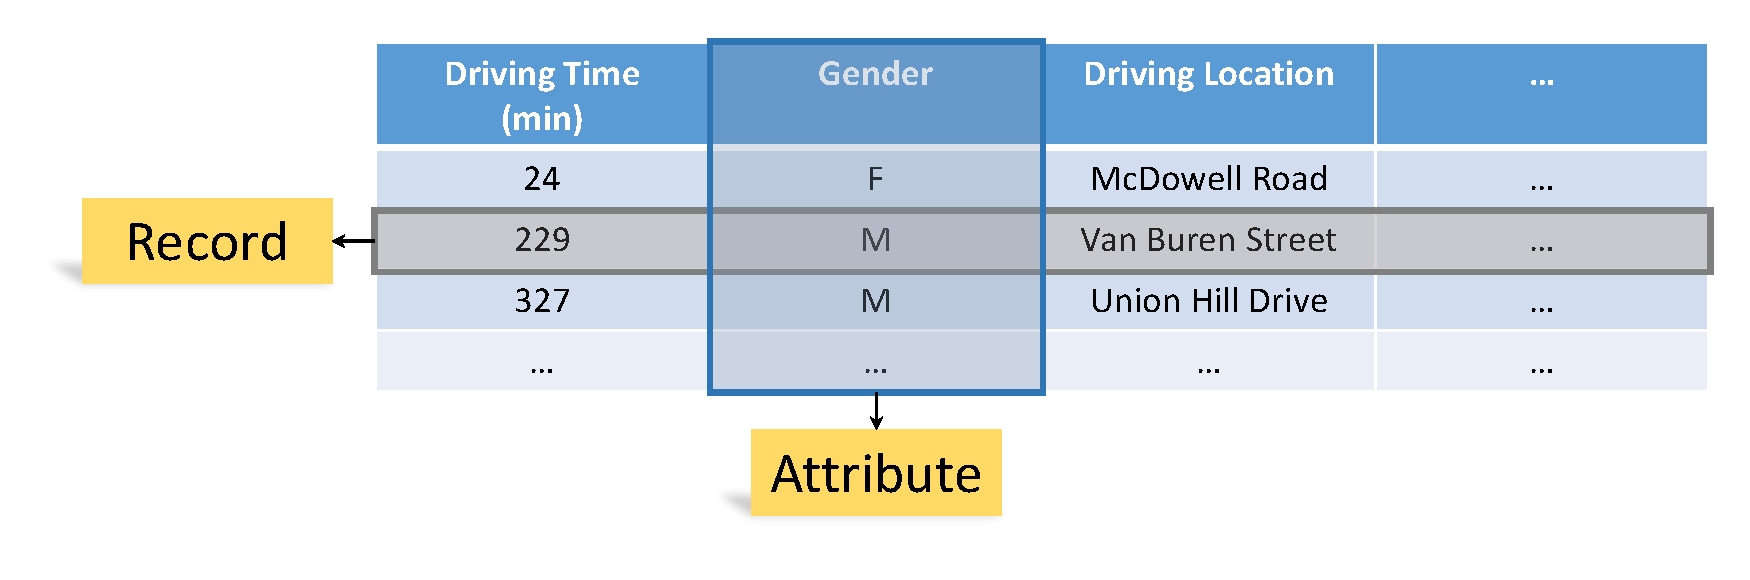
\includegraphics[width=0.9\textwidth]{chapter3/attr_pre}
  %\noindent\rule[0.25\baselineskip]{0.4855\textwidth}{0.95pt}
  \bicaption[fig:attr_pre]{的士司机行车记录数据集}{的士司机行车记录数据集}{Fig}{An illustration of taxi drivers' driving dataset}
\end{figure}

在图\ref{fig:attr_pre}中,我们可以看到该数据集有许多的属性,比如行车时间、司机性别以及行驶地点等等。这些属性的值可以是数值型的,也可以是文字性的。如果数据卖家想基于这些数据的信息量给这个数据集定价,那么其首要问题是弄起初这个数据集含有多少的信息量。因此,我们首要目标是去找到一个合适的方法精确度量该数据集所含有的信息量。在得到了该数据集的信息量之后,我们需要将其映射到一个合适的价格。

用更加形式化的方式叙述上述问题,对于一个有着$m$个属性和$n$条记录的数据集$\bm{D}$,它能表示成一个矩阵$\bm{X}$:
\begin{equation}
\bm{X}=
\left(
\begin{matrix}
 x_{11}      &  x_{12}      & \cdots &  x_{1m}      \\
 x_{21}     &  x_{22}      & \cdots &  x_{2m}      \\
 \vdots & \vdots & \ddots & \vdots \\
  x_{n1}      &  x_{n2}      & \cdots &  x_{nm}      \\
\end{matrix}
\right).
\end{equation}

在矩阵$\bm{X}$中,行向量$\bm{r_i}$表示原数据集中一条记录:
\begin{equation}
\bm{r_i}=\left(
\begin{matrix}
 x_{i1},      &x_{i2},      &\cdots, &x_{im}      \\
\end{matrix}
\right),
\end{equation}

其中,$i=1,...,n$。令$\bm{R}$表示一组记录$\{\bm{r_{i_1}},\bm{r_{i_2}},...,\bm{r_{i_k}}\}$的集合。类似的,列向量$\bm{c_j^\mathrm{T}}$表示原数据集中的一列属性:
\begin{equation}
 \bm{c_j^\mathrm{T}}=\left(
\begin{matrix}
 x_{1j};     &x_{2j};      &\cdots; &x_{nj}      \\
\end{matrix}
\right),
\end{equation}

其中,$j=1,...,m$。同样地,令$\bm{C}$表示一组属性$\{\bm{c_{j_1}},\bm{c_{j_2}},...,\bm{c_{j_k}}\}$的集合。需要指出的是,$\bm{r_i}$中的每个元素的值可以是不同类型的,比如数值、文字、日期等。但是$\bm{c_j}$的元素的值必须是同一类型的。

那么基于信息量的给数据集$\bm{D}$定价的方法可以分为两步:1)量化地度量数据集$\bm{D}$或其子集的信息量$H$;2)基于度量结果,找到一个合适的函数$l(\dot)$,将信息量$H$映射到一个价格$pr$,即$pr=l(H(\bm{D}))$。

为了达到上述目标,在下文中我们首先提出一个基于信息熵的信息量检测方法。然后基于检测结果,我们给出一个定价模型。

\subsection{数据商品信息量的测量}
在本小节中,我们先定义了元组和元组集合。然后,我们基于信息熵\cite{shannon2001mathematical}给出了相应的信息测量方法。

\begin{defn}[元组]
 对于给定的一个数据集$\bm{D}$,元组$\bm{t}$被定义为$\bm{D}$中一条记录$\bm{r}$的非空子集,即$\bm{t} \subseteq \bm{r}$且$\bm{t} \ne \emptyset$。
\end{defn}

\begin{defn}[元组集合]
元组集合$Tup$是一系列元组$\{\bm{t_{i_1}},\bm{t_{i_2}},...,\bm{t_{i_k}}\}$的集合。因此,$Tup$也是数据集$\bm{D}$的非空子集,即$Tup \subseteq \bm{D}$ 且 $Tup \ne \emptyset$。
\label{def:tuple_set}
\end{defn}

对于定义\ref{def:tuple_set},元组集合$Tup$可以是数据集的子集也可以就是数据集本身。实际上,元组集合是本文提出信息测量方法的最小单元。以下四个信息熵测量指标都是基于元组的。

\begin{defn}[数据信息熵]
对于一个有着$n$条元组$\{\bm{t_i}$$|i=1,...,n\}$的元组集合$Tup$,其数据信息熵$H_{ind}$定义为:
\begin{equation}
  H_{ind}(Tup)=-\sum_{\bm{t_i} \in Tup}p(\bm{t_i})\log_{b}p(\bm{t_i}),
  \label{eq:data_individual_entropy}
\end{equation}
\label{def:data_individual_entropy}
\end{defn}
其中,$b$是公式\ref{eq:data_individual_entropy}中对数的基。信息常用度量单位为比特,当对数基底$b$取为$2$时。除非特别指出,下文所有的对数都指的是以$2$为基底的对数,即$\log_2x$。数据信息熵是本文提出数据信息测量方法的最基础概念,它能测量出单个元组集合的信息量。

\begin{defn}[数据联合熵]

对于有$n_1$条元组的元组集合$Tup_1$和有$n_2$条元组的元组集合$Tup_2$,它们的数据联合熵$H_{joint}$定义为:

\begin{equation}\label{eq:joint_entropy}
  \begin{aligned}
    H_{joint}(Tup_1,Tup_2)=-\sum_{\bm{t_i} \in Tup_1} \sum_{\bm{t_j} \in Tup_2} p(\bm{t_i},\bm{t_j}) \log p(\bm{t_i},\bm{t_j})。
  \end{aligned}
\end{equation}

\label{def:data_joint_entropy}
\end{defn}

需要指出的是数据联合熵是可以轻易地扩展到多个元组集合的信息测量。

\begin{defn}[数据条件熵]
对于有$n_1$条元组的元组集合$Tup_1$和有$n_2$条元组的元组集合$Tup_2$,那么在已知$Tup_1$的条件下$Tup_2$的信息熵被定义为
\begin{equation}\label{eq:conditional_entropy}
  \begin{aligned}
    H_{cond}(Tup_2|Tup_1)=-\sum_{\bm{t_i} \in Tup_1} \sum_{\bm{t_j} \in Tup_2} p(\bm{t_i},\bm{t_j})\log p(\bm{t_j}|\bm{t_i}),
  \end{aligned}
\end{equation}
\label{def:data_conditional_entropy}
\end{defn}
其中$H_{cond}(Tup_2|Tup_1)=0$,当且仅当$Tup_2$被$Tup_1$完全决定。换句话说,一旦$Tup_1$已知,$Tup_2$就被唯一确定了。相反的情况是,$H_{cond}(Tup_2|Tup_1)=H_{ind}(Tup_2)$当且仅当$H_{ind}(Tup_1)$和$H_{ind}(Tup_2)$是统计独立的,换句话说就是即使$Tup_1$已知,也不能获得$Tup_2$的任何信息。

\begin{defn}[数据互信息]
对于有$n_1$条元组的元组集合$Tup_1$和有$n_2$条元组的元组集合$Tup_2$,$Tup_1$和$Tup_2$的数据互信息$I$定义为:

\begin{equation}
\label{eq:mutual_information}
  \begin{aligned}
    I(Tup_1;Tup_2)=\sum_{\bm{t_i} \in Tup_1} \sum_{\bm{t_j} \in Tup_2} p(\bm{t_i},\bm{t_j}) \log\frac{p(\bm{t_i},\bm{t_j})}{p(\bm{t_i})p(\bm{t_j})}。
  \end{aligned}
\end{equation}

\label{def:data_mutal_information}
\end{defn}


相比于数据条件熵,数据互信息是被用来度量两个元组的依赖程度。

需要指出的是,元组的元素也可以是连续型数值的。然而上述定义的相关熵都是默认元组元素是离散的。以上定义可以通过将求和符号替换为积分符号后扩展到连续型元组上:

\begin{equation}
  H_{ind}(Tup)=-\int_{\bm{t_i} \in Tup}p(\bm{t_i})\log p(\bm{t_i}),
\end{equation}
\begin{equation}
  H_{joint}(Tup_1,Tup_2)=-\int_{\bm{t_i} \in Tup_1} \int_{\bm{t_j} \in Tup_2} p(\bm{t_i},\bm{t_j}) \log p(\bm{t_i},\bm{t_j}),
\end{equation}
\begin{equation}
  H_{cond}(Tup_2|Tup_1)=-\int_{\bm{t_i} \in Tup_1} \int_{\bm{t_j} \in Tup_2} p(\bm{t_i},\bm{t_j})\log p(\bm{t_j}|\bm{t_i}),
\end{equation}
\begin{equation}
  I(Tup_1;Tup_2)=\int_{\bm{t_i} \in Tup_1} \int_{\bm{t_j} \in Tup_2} p(\bm{t_i},\bm{t_j}) \log\frac{p(\bm{t_i},\bm{t_j})}{p(\bm{t_i})p(\bm{t_j})}.
\end{equation}

然而,对于连续型变量而言,通常是很难确定其概率密度函数。另一方面,在计算机中积分的数值计算也是存在误差的。因此,计算连续型数据的数据信息熵的一般方法是将连续的输入空间切分为若干个离散的子空间,然后按照离散型变量计算其信息熵然。然而这种方法的内部误差会降低计算最后的熵的精确度,那么这就会影响定价策略。对于那些连续型、离散型数据均有的元组,其相应数据信息熵的计算方法是我们未来的工作之一。

此外,\cite{shannon2001mathematical}还列出一系列熵的性质,后续定价函数的讨论涉及到这些性质,因此我们简单陈述下相关性质。

\begin{propt}[数据信息熵的非负性]
\label{pr:entropry_non_negativity}
给定两个元组集合$Tup_1$和$Tup_2$,我们有

\begin{equation}
  H_{ind}(Tup_1)\ge 0, H_{ind}(Tup_2)\ge 0,
\end{equation}
\begin{equation}
  H_{joint}(Tup_1,Tup_2)\ge 0,
\end{equation}
\begin{equation}
  H_{cond}(Tup_1|Tup_2)\ge 0, H_{cond}(Tup_2|Tup_1)\ge 0,
\end{equation}
\begin{equation}
  I(Tup_1;Tup_2)\ge 0.
\end{equation}


性质\ref{pr:entropry_non_negativity}的证明如下:
\begin{proof}
首先来关注数据信息熵,$H_{ind}(Tup)$,其定义如下:

\begin{equation}
    H_{ind}(Tup)=-\sum_{\bm{t_i} \in Tup}p(\bm{t_i})\log p(\bm{t_i})。
    \label{proof:individual_entropy}
\end{equation}

由于 $0\le p(\bm{t_i}) \le 1$,那么

\begin{equation}
\log p(\bm{t_i}) \le 0。
\end{equation}

因此,根据公式(\ref{proof:individual_entropy}), $H_{ind}(Tup)$ 一定是非负的。

$H_{joint}(\cdot)$,$H_{cond}(\cdot)$, $H_{cond}(\cdot)$以及$I(\cdot)$的非负性同样可以采用上述类似步骤证明。

\end{proof}
\end{propt}

\begin{propt}[不同数据信息熵之间的关系]
给定两个元组集合$Tup_1$和$Tup_2$,我们有

\begin{equation}
\label{pr:entropry_relationships}
  H_{joint}(Tup_1,Tup_2)\le H_{ind}(Tup_1)+H_{ind}(Tup_2),
\end{equation}
\begin{equation}
  H_{joint}(Tup_1,Tup_2)\ge H_{ind}(Tup_1),
\end{equation}
\begin{equation}
  H_{joint}(Tup_1,Tup_2)\ge H_{ind}(Tup_2).
\end{equation}

性质\ref{pr:entropry_relationships}的证明如下:
\begin{proof}


首先从数据互信息的定义入手:

\begin{equation}
    I(Tup_1;Tup_2)=\sum_{\bm{t_i} \in Tup_1} \sum_{\bm{t_j} \in Tup_2} p(\bm{t_i},\bm{t_j}) \log\frac{p(\bm{t_i},\bm{t_j})}{p(\bm{t_i})p(\bm{t_j})}.
    \label{app:mutual_information}
\end{equation}


公式(\ref{app:mutual_information})能被重写为:
\begin{equation}
    \begin{aligned}
    I(Tup_1;Tup_2)&=\sum_{\bm{t_i} \in Tup_1} \sum_{\bm{t_j} \in Tup_2} p(\bm{t_i},\bm{t_j}) [\log p(\bm{t_i},\bm{t_j})\\
    &- \log p(\bm{t_i}) - \log p(\bm{t_j})]\\
    &=\sum_{\bm{t_i} \in Tup_1} \sum_{\bm{t_j} \in Tup_2} p(\bm{t_i},\bm{t_j})\log p(\bm{t_i},\bm{t_j})\\
    &-\sum_{\bm{t_i} \in Tup_1} \sum_{\bm{t_j} \in Tup_2} p(\bm{t_i},\bm{t_j})\log p(\bm{t_i})\\
    &-\sum_{\bm{t_i} \in Tup_1} \sum_{\bm{t_j} \in Tup_2} p(\bm{t_i},\bm{t_j})\log p(\bm{t_j}).
    \end{aligned}
    \label{eq:mutal_information_rewrite1}
\end{equation}

根据定义\ref{def:data_individual_entropy}和定义\ref{def:data_joint_entropy},公式~(\ref{eq:mutal_information_rewrite1}) 能进一步写成:

\begin{equation}
\begin{aligned}
    H_{joint}(Tup_1,Tup_2)&=H_{ind}(Tup_1)+H_{ind}(Tup_2)\\
    &-I(Tup_1;Tup_2).
\label{eq:mutal_information_rewrite2}
\end{aligned}
\end{equation}

由于数据信息熵和数据互信息的非负性,我们有:

\begin{equation}
  H_{joint}(Tup_1,Tup_2)\le H_{ind}(Tup_1)+H_{ind}(Tup_2),
\end{equation}

另一方面,根据定义\ref{def:data_individual_entropy},定义\ref{def:data_joint_entropy},以及定义\ref{def:data_conditional_entropy}, 公式(\ref{eq:mutal_information_rewrite1})能进一步写成:
\begin{equation}
    H_{joint}(Tup_1,Tup_2)=H_{cond}(Tup_1|Tup_2)+H_{ind}(Tup_2),
\end{equation}
\begin{equation}
    H_{joint}(Tup_1,Tup_2)=H_{cond}(Tup_2|Tup_1)+H_{ind}(Tup_1).
\end{equation}

类似地,由于数据信息熵的非负性,那么有:

\begin{equation}
  H_{joint}(Tup_1,Tup_2)\ge H_{ind}(Tup_1),
\end{equation}
\begin{equation}
  H_{joint}(Tup_1,Tup_2)\ge H_{ind}(Tup_2).
\end{equation}

\end{proof}
\end{propt}


\subsection{通用定价模型}

在本小节中,我们提出了一个基于数据信息熵的通用定价模型,而不是给出一个具体的定价函数。此外,该定价模型的相关性质和优点在本小节中也会进行讨论。

\begin{defn}[定价函数]
对一个给定的数据集$\bm{D}$,定价函数${pr(\bm{D})}:\bm{D}\to \mathbb{R^{+}}$, 其中 $\mathbb{R^{+}}$ 非负实数。一个基于数据信息熵的定价函数是:
\begin{equation}
  pr(\cdot) \equiv l(H(\cdot)),
  \label{eq:pricing_function}
\end{equation}
其中$l(\cdot)$ 是一个非递减的联系函数,它应该满足如下条件:
\begin{equation}
\forall x_1 \ge x_2, l(x_1) \ge l(x_2),
\label{eq:link_function_property1}
\end{equation}
\begin{equation}
\forall x_1, x_2 \ge 0, l(x_1+x_2) \le l(x_1)+l(x_2).
\label{eq:link_function_property2}
\end{equation}
\end{defn}

\begin{exmp}
对于两个数据集$\bm{D_1}$和$\bm{D_2}$以及一个基于数据信息熵的定价函数$pr(\cdot) \equiv l(H(\cdot))$,如果$H(\bm{D_1})\ge H(\bm{D_2})$,那么有$pr(\bm{D_1})\ge pr(\bm{D_2})$。
\end{exmp}

为了陈述简洁,上述数据信息熵的定价函数都指的是数据独立信息熵或者数据联合熵,取决于$H(\cdot)$中参数个数。选择具体的定价函数要取决于具体的市场情况,这也是本文的未来工作之一。

\begin{propt}[定价函数的非负性]
定价函数的输出一定是大于零的,即$pr(\cdot) \ge 0$总是成立。
\label{pr:pricing_function_pr_1}
\end{propt}

定价函数的非负性是显然的,因为数据卖家在出售商品的同时还倒贴钱给数据买家。接下来,基于数据信息熵的定价函数的\textit{无套利}性质会被讨论,这个性质也是其最大的优点。为了详细地讨论这个性质,我们首先要介绍下一个数据集中的操作,即\textit{连接}。

\begin{defn}[数据集连接]

给定两个数据集$\bm{D_1}$和$\bm{D_2}$,$\bm{D_1}$有$n_1$条记录$\bm{R_1}$和$m_1$条属性$\bm{C_1}$,$\bm{D_2}$有$n_2$条记录$\bm{R_2}$和$m_2$条属性$\bm{C_2}$,$\bm{D_1}$和$\bm{D_2}$的连接$\bm{D_J}$定义为:

\begin{equation}
\bm{D_J}=\bm{D_1} \circledcirc \bm{D_2}.
\end{equation}
\end{defn}

这里给出数据连接操作的两个例子:

\begin{case}
如果在数据集$\bm{D_1}$和$\bm{D_2}$中没有共同的属性,即$\bm{C_1} \cap \bm{C_2} = \emptyset$,那么它们的连接$\bm{D_J}$就会有$n_1+n_2$条记录和$m_1+m_2$条属性。

\end{case}

\begin{case}
如果在数据集$\bm{D_1}$和$\bm{D_2}$中有共同的属性,即$\bm{C_1} \cap \bm{C_2} \ne \emptyset$,那么它们的连接$\bm{D_J}$就会有$n_1+n_2$条记录和$\|\bm{C_1} \cup \bm{C_2}\|$ 条属性。

\end{case}

数据集\textit{连接}的操作能被扩展到多个数据集的情况。如果有多个数据集 $\bm{D_1,D_2,...,D_k}$,我们把他们的连接集合记为$\bm{D_J}=\circledcirc_{i=1}^k \bm{D_i}$。值得注意的是这里的连接操作不同于SQL类的数据库连接操作。为了更加直观地说明这个连接操作,我们举出了如下例子:

\begin{exmp}
数据集$\bm{D_1}$有$3$条记录和$3$个属性$\{a,b,c\}$,数据集$\bm{D_2}$有$4$条记录和$2$个属性$\{c,d\}$。它们的连接数据集$\bm{D_1} \circledcirc \bm{D_2}$将会有$7$条记录和$4$个属性$\{a,b,c,d\}$,如图\ref{fig:joint_data_set}所示。在连接数据集中,那些非共同属性的缺失值是用'\#'填满。
\end{exmp}

\begin{figure}[h]
  \centering
    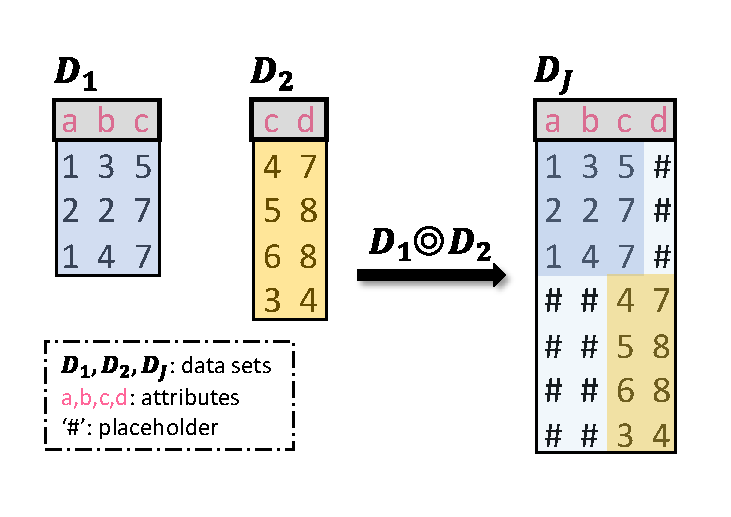
\includegraphics[width=0.7\textwidth]{chapter3/joint_data_set}
  %\noindent\rule[0.25\baselineskip]{0.4855\textwidth}{0.95pt}
  \bicaption[fig:joint_data_set]{数据集连接操作示意图}{数据集连接操作示意图}{Fig}{An illustration of dataset join}
\end{figure}

\subsection{讨论}

\section{实验与评估}

\subsection{实践中遇到的问题}

\subsection{在公开研究数据集上的实验}

\subsection{在大规模工业数据集上的实验}

\subsection{定价函数}

\section{本章小结}